\documentclass[tikz,border=10pt]{standalone}
\usetikzlibrary{positioning}
\usepackage{amsmath,amssymb}

\begin{document}
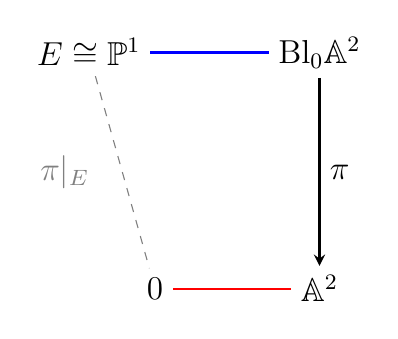
\begin{tikzpicture}[
    >=stealth,
    every node/.style={font=\large}
]

% Blow-up space (top)
\node (Bl) at (0,3) {$\mathrm{Bl}_0\mathbb{A}^2$};

% Original space (bottom)
\node (A2) at (0,0) {$\mathbb{A}^2$};

% Blow-down map
\draw[->, thick] (Bl) -- (A2) node[midway, right] {$\pi$};

% Exceptional curve in blow-up
\node[left=1.5cm of Bl] (E) {$E \cong \mathbb{P}^1$};
\draw[thick, blue] (E) -- (Bl);

% Origin in A^2
\node[left=1.5cm of A2] (O) {$0$};
\draw[thick, red] (O) -- (A2);

% Vertical dashed line connecting E to 0
\draw[dashed, gray] (E) -- (O) node[midway, left, xshift=-0.3cm] {$\pi|_E$};

\end{tikzpicture}
\end{document}
